\documentclass{article}
\usepackage{graphicx} % Required for inserting images
\usepackage{tikz}
\usepackage{amsmath}

\title{Readout waveform limits}
\author{}
\date{}

\begin{document}

%\maketitle

\section{Maximum readout area}
See Figs. \ref{fig:se} \& \ref{fig:gre}. 
We wish to find the maximum readout area $A$, given the readout duration $d$, and the slew rate $s$.
For both spin echo and gradient echo, the following holds:
\begin{equation}
    A = dg
    \label{eq:readArea}
\end{equation}
\begin{equation}
    B = g^2/{2s} = A^2/{2d^2 s}
    \label{eq:slewArea}
\end{equation}
where $g$ is the readout gradient amplitude.

\subsection{Spin echo}
See Fig. \ref{fig:se}. 
We seek the maximum readout area $A=\min(A_r, A_p)$, where $A_r$ is limited by the available time $t_r$ corresponding to half the readout gradient: 
\begin{equation}
    \begin{split}
        t_r & = d/2 + g/s = d/s + A_r / {ds} \\
        A_r & = dst_r-d^2s/2, 
    \end{split}
    \label{eq:halfReadoutTime}
\end{equation}
and $A_p$ is limited by the maximum prephaser duration $t_p$:
\begin{equation}
    A_p/2 + B = h(t_p-h/s),
\end{equation}
where $h$ is the prephaser peak amplitude. 
If the prephaser is triangular, then
\begin{equation}
    h = st_p/2.
    \label{eq:SEprephaserAmp}
\end{equation}
If $h>g_{max}$, we let $h=g_{max}$, which corresponds to a trapezoid prephaser waveform.
The prepahser-limited area can then be found:
\begin{equation}
    \begin{split}
        0 & = A_p^2/{2d^2 s} - (h(t_p-h/s)-A_p/2) \\
          & = A_p^2 + d^2sA_p+2d^2h(h-st_p) \\
      A_p & = d(\sqrt{d^2s^2 - 8h(h-st_p)} - ds)/2 \\
    \end{split}
    \label{eq:prephaserLimitedArea}
\end{equation}

\begin{figure}[h]
    \centering
    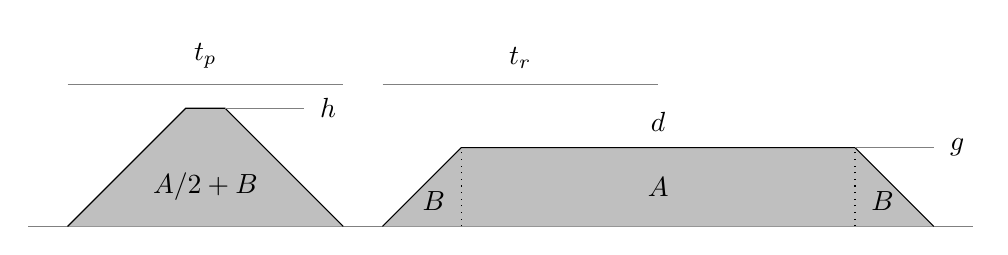
\begin{tikzpicture}[x=1mm, y=1mm, inner sep=2mm]
        \draw[gray]  (0, 0) -- (120, 0); % axis
        \draw[fill=lightgray] (5, 0) -- (20, 15) -- (25, 15) -- (40, 0);  % prephaser
        \draw[gray] (25, 15) -- (35, 15) node[right, black] {$h$}; % prephaser amplitude
        \draw (22.5, 5) node {$A/2+B$}; % prephaser area
        \draw[gray] (5, 18) -- (40, 18) node[midway, above, black] {$t_p$}; % availble prephaser time
        \draw[fill=lightgray] (45, 0) -- (55, 10) -- (105, 10) node[midway, above] {$d$} -- (115, 0); % readout
        \draw[gray] (45, 18) -- (80, 18) node[midway, above, black] {$t_r$}; % half readout gradient time
        \draw[gray] (105, 10) -- (115, 10) node[right, black] {$g$}; % readout amplitude
        \draw (80, 5) node {$A$}; % readout area
        \draw[dotted] (55, 0) node[anchor=south east] {$B$} -- (55, 10); % readtrap slew area
        \draw[dotted] (105, 0) node[anchor=south west] {$B$} -- (105, 10); % readtrap slew area
    \end{tikzpicture}
    \caption{Spin echo prephaser and readout gradient}
    \label{fig:se}
\end{figure}

\subsection{Gradient echo}

See Fig. \ref{fig:gre}. 
For gradient echo, the maximum readout area $A$ is limited by the time $t$ between the end of excitation and $TE$:
\begin{equation}
    A/2 + B = h(t-d/2-g/s-h/s)
    \label{eq:grePrephaserArea}
\end{equation}
where $h$ is the prephaser peak amplitude. 
We wish to determine $h$ under the assumption that the prephaser is triangular:
\begin{equation}
    t = 2h/s+g/s+d/2
    \label{eq:greTriangleT}
\end{equation}

It follows from eqs. \ref{eq:readArea}, \ref{eq:slewArea}, \ref{eq:grePrephaserArea}, and \ref{eq:greTriangleT} that
\begin{equation}
    \begin{split}
        0 & = 8h^2 - 16sth + s^2(4t^2-d^2) \\
        h & = s (t - \sqrt{t^2/2+d^2/8}) \\
    \end{split}
    \label{eq:GREprephaserAmp}
\end{equation}
If $h>g_{max}$, we set $h=g_{max}$, which corresponds to a trapezoid prephaser waveform. 
The maximum area is can then be found:
\begin{equation}
    \begin{split}
        0 & = A^2 + Ad(ds+2h) + 2d^2h(h-s(t-d/2)) \\
        A & = d(\sqrt{(ds+2h)^2-8h(h-s(t-d/2))} - ds - 2h)/2
    \end{split}
    \label{eq:greArea}
\end{equation}

\subsection{Gradient echo EPI}
For EPI, eq. \ref{eq:grePrephaserArea} can be replaced by:
\begin{equation}
    A/2 + B = h(t-N(d+v)-Mg/s-h/s+v/2)
    \label{eq:greEPIprephaserArea}
\end{equation}
where $N$ and $M$ are the number of readouts and readout ramps up to $TE$, and $v$ is the gap duration between readouts. 
Then, it follows from eqs. \ref{eq:readArea}, \ref{eq:slewArea}, \ref{eq:greTriangleT}, and \ref{eq:greEPIprephaserArea} that $h$ may be calculated as
\begin{equation}
    0 = 8h^2(3-2M) + 4 hs (t(2M-6)+d(2N-M)+v(2N-1)) + s^2(4t^2-d^2)
    \label{eq:GREEPIprephaserAmp}
\end{equation}
After truncating to $g_{max}$, $A$ can be calculated as
\begin{equation}
    0 = A^2 + Ad(ds+2Mh) + d^2h(2h-s(2t-2N(d+v)+v))
    \label{eq:greEPIArea}
\end{equation}

In case the duration of the read prephaser plus readut rampup is shorter than either the phaser or the slice selection gradient rampdown plus the slice rephaser, the area will be limited by $q$, defined as the available time from readout plateu start to $TE$:
\begin{equation}
    q = Nd + (M-1) g/s
    \label{eq:q}
\end{equation}
which implies that
\begin{equation}
    A = \frac{ds(q - N(d+v) + v/2)}{M-1}
    \label{eq:qArea}
\end{equation}

\begin{figure}
    \centering
    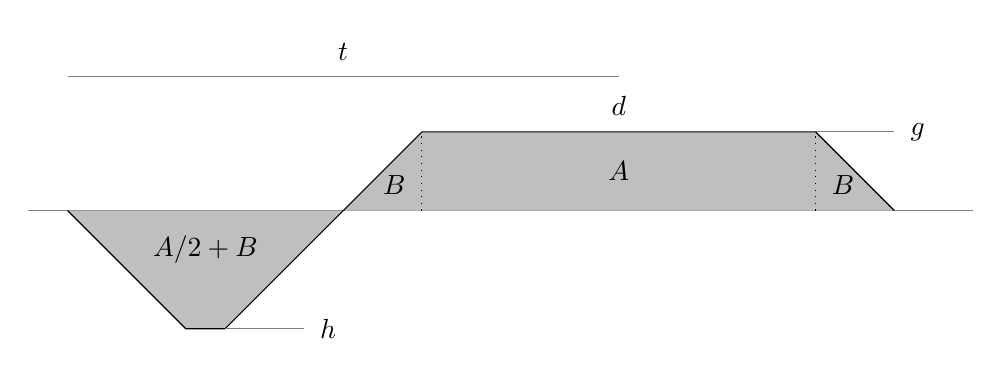
\begin{tikzpicture}[x=1mm, y=1mm, inner sep=2mm]
        \draw[gray]  (0, 0) -- (120, 0); % axis
        \draw[fill=lightgray] (5, 0) -- (20, -15) -- (25, -15) -- (40, 0);  % prephaser
        \draw[gray] (25, -15) -- (35, -15) node[right, black] {$h$}; % prephaser amplitude
        \draw (22.5, -5) node {$A/2+B$}; % prephaser area
        \draw[gray] (5, 17) -- (75, 17) node[midway, above, black] {$t$}; % availble time
        \draw[fill=lightgray] (40, 0) -- (50, 10) -- (100, 10) node[midway, above] {$d$} -- (110, 0); % readout
        \draw[gray] (100, 10) -- (110, 10) node[right, black] {$g$}; % readout amplitude
        \draw (75, 5) node {$A$}; % readout area
        \draw[dotted] (50, 0) node[anchor=south east] {$B$} -- (50, 10); % readtrap slew area
        \draw[dotted] (100, 0) node[anchor=south west] {$B$} -- (100, 10); % readtrap slew area
    \end{tikzpicture}
    \caption{Gradient echo with trapezoid prephaser}
    \label{fig:gre}
\end{figure}

\newpage
\section{Readout duration limits}
We wish to find limits on the readout duration $d$, given the readout area $A$ and the slew rate $s$.

\subsection{Spin echo}
See Fig. \ref{fig:se}. 
The maximum readout duration $d_{max}$, is limited by the available time $t_r$ corresponding to half the readout gradient according to eq. \ref{eq:halfReadoutTime}:
\begin{equation}
    \begin{split}
        0 & = d_{max}^2-2td_{max}+2A/s \\
        d_{max} & = t_r \pm \sqrt{t_r^2-2A/s}
    \end{split}
\end{equation}

The minimum readout duration $d_{min}$ is determined by the time available for the prephaser and follows from eq. \ref{eq:prephaserLimitedArea}:
\begin{equation}
    \begin{split}
        0 = d_{min}^2(sA+2h(h-st_p)) + A^2 \\
        d_{min} = \sqrt{A^2/(2hst_p - sA - 2h^2)} \\
    \end{split}
\end{equation}
where $h$ is given by eq. \ref{eq:SEprephaserAmp}, truncated to $g_{max}$ (trapezoid prephaser). 

\subsection{Gradient echo}
See Fig. \ref{fig:gre}. 
Using eqs. \ref{eq:readArea}, \ref{eq:slewArea}, \ref{eq:grePrephaserArea}, and assuming a triangular prephaser gradient (eq. \ref{eq:greTriangleT}):
\begin{equation}
    A/2 + A^2/{2d^2 s} = h^2/s
\end{equation}
Remains to solve for $h$ and then find $d$ as function of $\min(g_{max}, h)$.

\newpage

\section{Minimum slice thickness}

\subsection{Gradient echo}
We can reuse Fig. \ref{fig:gre}; by reversing the time axis it can represent the excitation pulse slice selection gradient and slice rephaser. 
In this case, $t$ represents the time between the isodelay point of the excitation pulse ($t=0$) and the start of the signal readout. 
We can then find the amplitude of the triangular slice rephaser, $h$, from Eq. \ref{eq:GREprephaserAmp} and truncate it to $g_{max}$.
The minimum slice thickness $T$ is then
\begin{equation}
    T = \frac{B_e d}{\gamma A}
    \label{eq:sliceThickness}
\end{equation}
where $B_e$ is the transmit bandwidth (FWHM) of the excitations pulse, $\gamma$ is the gyromagnetic ratio, and $A$ is given by eq. \ref{eq:greArea}.

\subsection{Spin echo}
The spin echo case is similar to gradient echo, but we now define $t$ as the time between the isodelay point of the excitation pulse and the start of the refocusing pulse. 
This time additionally needs to encompass the rise time of the refocusing pulse slice selection gradient with amplitude, which is assumed to equal that of the excitation slice selection amplitude $g$ (then, the relative slice thickness of the pulses is determined by their relative transmit bandwidths): 
\begin{equation}
    A/2 + B = h(t-d/2-h/s-2g/s)
    \label{eq:seSliceRephaserArea}
\end{equation}

Assuming a triangular slice rephaser gradient, we have
\begin{equation}
    t = d/2 + 2g/s + 2h/s
    \label{eq:seTriangleSliceRephaser}
\end{equation}

The slice rephaser peak amplitude follows from eqs. \ref{eq:readArea}, \ref{eq:slewArea}, \ref{eq:seSliceRephaserArea}, and \ref{eq:seTriangleSliceRephaser}:
\begin{equation}
    h = s(\sqrt{2(d + 2t)^2-4d^2}- d - 2t)/4
    \label{eq:GREprephaserAmp}
\end{equation}
After truncating $h$ to $g_{max}$, $A$ follows from eqs. \ref{eq:readArea}, \ref{eq:slewArea}, and \ref{eq:seSliceRephaserArea}:
\begin{equation}
    %A = \left( \sqrt{(d(ds + 4h))^2-4d^2h(ds+2h-2st)}-d(ds + 4h) \right)/2
    A = \frac{\sqrt{(d(ds + 4h))^2-4d^2h(ds+2h-2st)}-d(ds + 4h)}{2}
    \label{eq:GREprephaserAmp}
\end{equation}
The minimum slice thickness is then given by eq. \ref{eq:sliceThickness}.

\end{document}